% !TeX spellcheck = en_US
% !TeX encoding = UTF-8
\documentclass{beamer}

\mode<presentation> { \usetheme{Madrid} }

\usepackage{graphicx, graphics}
\usepackage{apacite}
\usepackage[style=iso]{datetime2}
\usepackage{ulem}
\DeclareGraphicsExtensions{.pdf, .png, .jpg, .gif}

\title[Docker]{Docker Lecture}

\author{Jaewoong Lee}
\institute[UNIST]
{
    Ulsan National Institute of Science and Technology
    \medskip
    \newline
    \textit{jwlee230@unist.ac.kr}
}
\date{\today}

\begin{document}
    \begin{frame}
        \titlepage
    \end{frame}

    \begin{frame}
        \frametitle{Overview}
        \tableofcontents
    \end{frame}

    \section{Why Docker?}
    \begin{frame}
        \frametitle{Why Docker?}

        \begin{itemize}
            \item Change Server Environment
            \item Download \& Install again
            \item Occurs error, ask to maintainer...
        \end{itemize}

        \begin{figure}[h!]
            
\includegraphics[width=0.5 \linewidth]{figures/itworks.png}
        \end{figure}
    \end{frame}

    \section{Virtual Machine}
    \begin{frame}
        \frametitle{Virtual Machine?}

        \begin{itemize}
            \item Machine in the machine \sout{in the machine in the machine ...}
            \item Machine\textbf{s} in the machine
        \end{itemize}

        However, VM (Virtual Machine) is ...
        \begin{itemize}
            \item Slow...
            \item Virtualizing from CPU $\rightarrow$ still slow.
            \item VM needs 'Guest OS' $\therefore$ Performance leakage.
        \end{itemize}
    \end{frame}

    \section{Docker}
    \begin{frame}
        \frametitle{Docker}

        \begin{itemize}
            \item Does not require 'Guest OS'
            \item Sharing system call with Host OS
            \item (Almost) No performance leakage
        \end{itemize}

        \begin{figure}[h!]
            $\begin{array}{cc}
                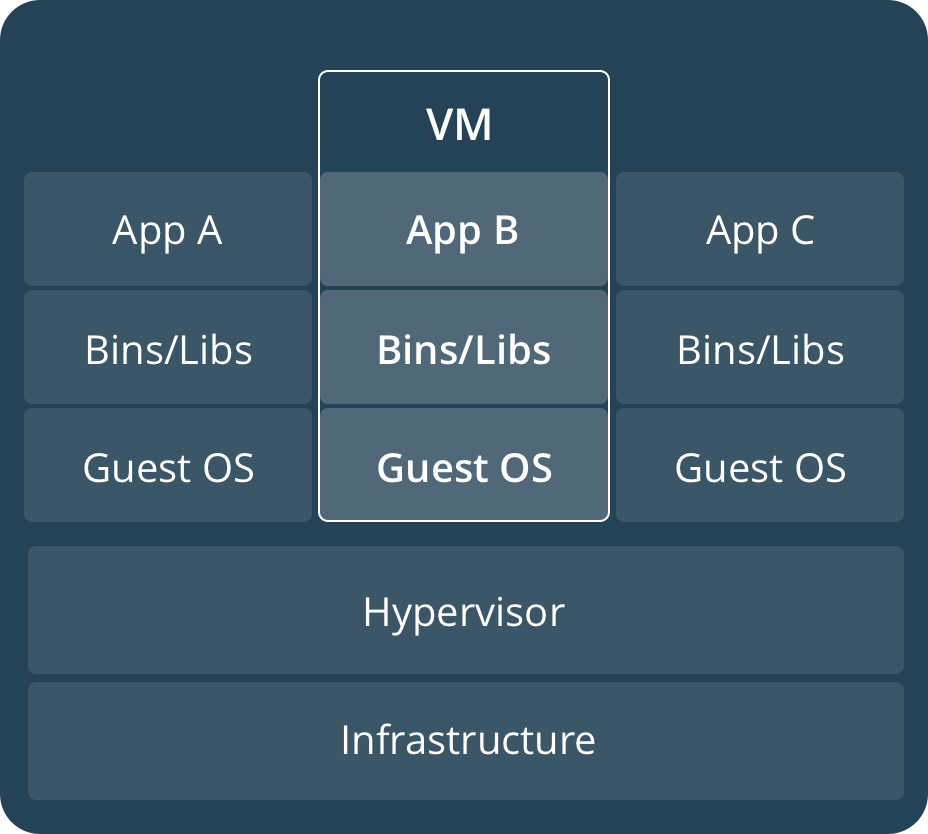
\includegraphics[width=0.3 \linewidth]{figures/vm.png}
                &
                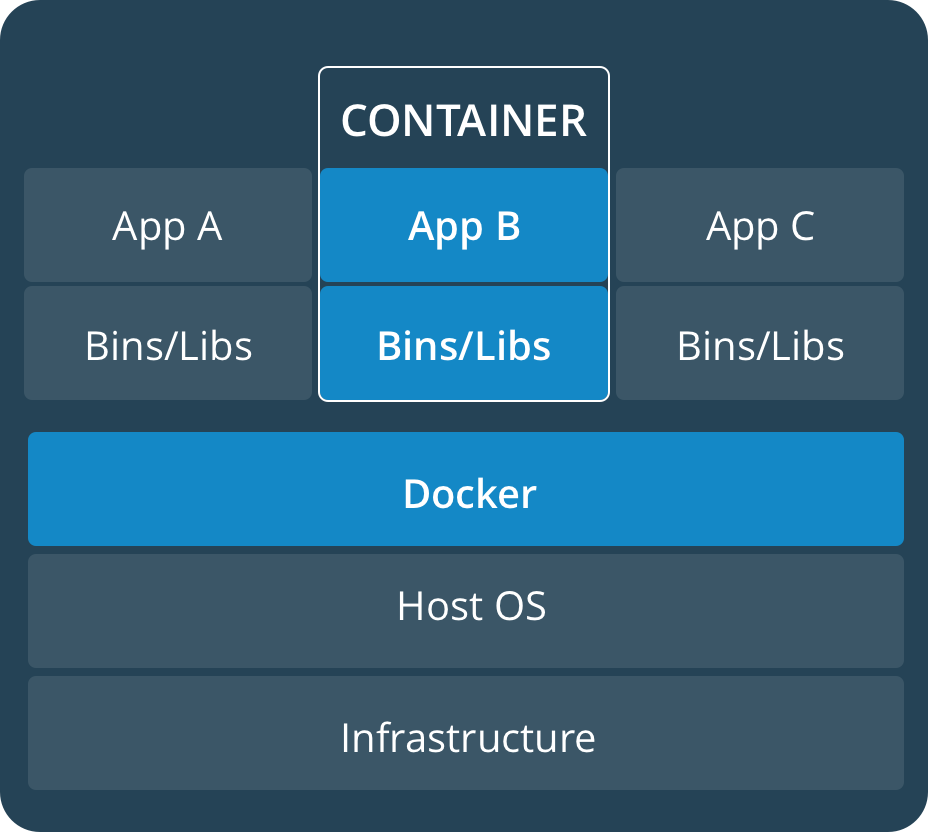
\includegraphics[width=0.3 \linewidth]{figures/docker.png}
                \\
                \mbox{(a) VM} & \mbox{(b) Docker}
            \end{array}$
            \caption{VM vs. Docker (Docker Docs)}
        \end{figure}
    \end{frame}

    \begin{frame}
        \frametitle{Docker Image \& Container}
    \end{frame}

    \section{Dockerfile}
\end{document}